\newpage
\section{Punto 2}

\textit{Resolver gráficamente, utilizando backtracking, el juego de ubicar 4 reinas en un tablero de 4x4.}\\


Como se puede ver en el grafo (en este caso un árbol) de la figura \ref{fig:4reinas} inicialmente se parte de que el vector se encuentra vació luego se sabe que cumplirá con las restricciones por lo que inserta la reina en la primer posición y crea un nuevo nodo (2) que verificara si se puede insertar una nueva reina, al encontrarse en el nivel 2 del árbol verificara si para la segunda fila del vector se puede insertar alguna reina, en este caso detecta que la columna 3 para la fila 2 cumple con la restricción por lo que inserta la posición de la reina y genera el nodo (3) el cual vuelve a realizar la verificación y se encuentra con que no hay una posición factible para insertar reinas por lo que el algoritmo vuelve al nodo padre de este (hace backtracking). Una vez en el nodo padre busca si es posible insertar una nueva reina en otra columna para la fila 2 y el algoritmo iterara hasta que se llegue a un vector solución o se verifiquen todas las posibles combinaciones.

\begin{figure}[!htb]
  \centering
  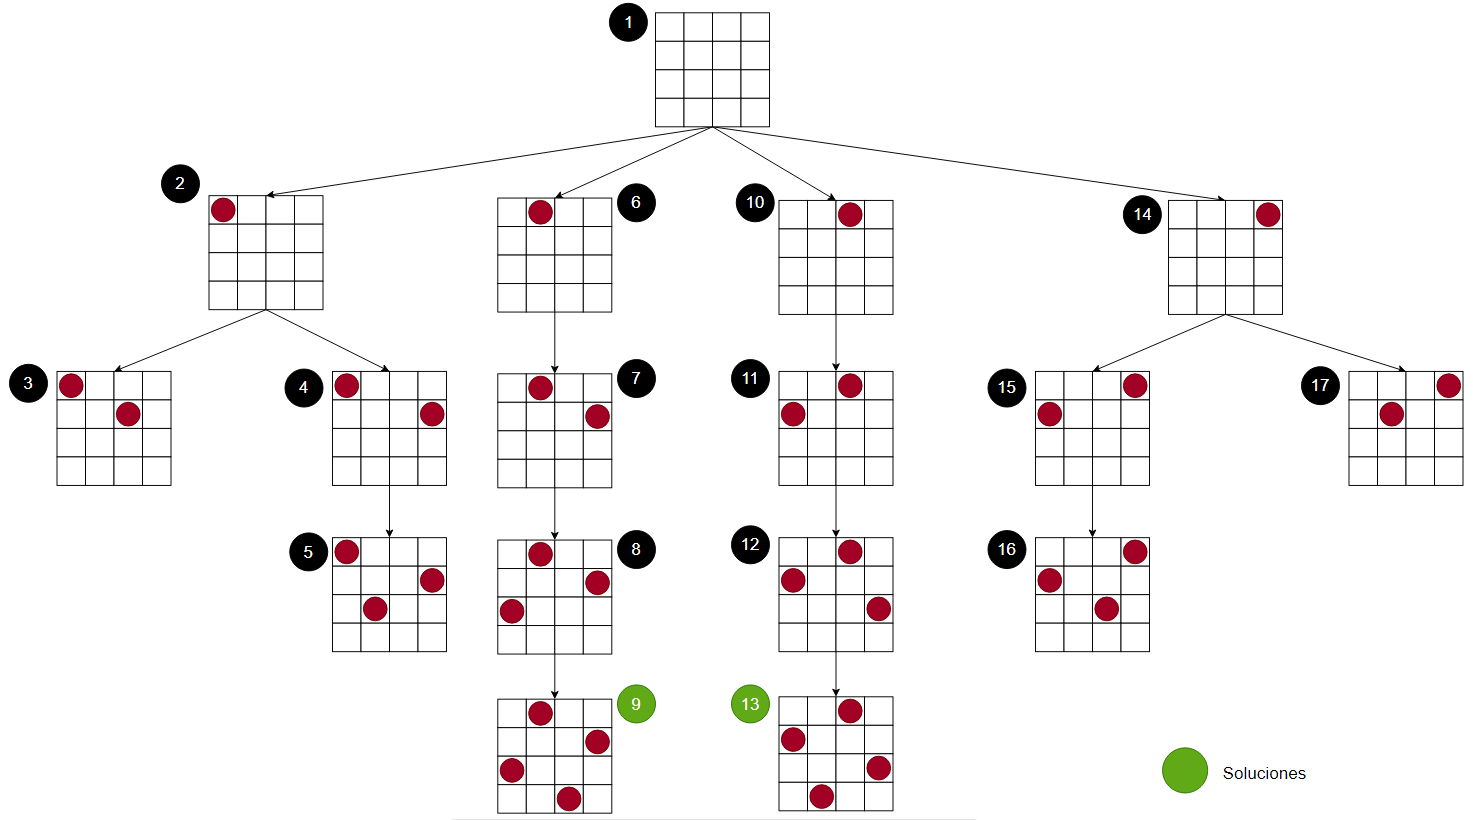
\includegraphics[width=\textwidth, scale=1]{Images/Punto2/4 reinas.png}
  \caption{Solución al problema de las 4 reinas para un tablero de 4x4}
  \label{fig:4reinas}
\end{figure}